\documentclass[12pt,a4paper]{article}
\usepackage[utf8x]{inputenc}
\usepackage{ucs}
\usepackage[spanish]{babel}
\usepackage{amsmath}
\usepackage{amsfonts}
\usepackage{amssymb}
\usepackage{makeidx}
\usepackage{graphicx}
\usepackage[hidelinks]{hyperref}
\usepackage[left=2cm,right=2cm,top=2cm,bottom=2cm]{geometry}
\author{Cervantes Martinez Luis Osvaldo\\Reyes Alvarez Ulises Isaac\\4.B Ing. Mecatrónica\\Mtro. Carlos Enrique Morán Garabito\\Sistemas Electrónicos de Interfaz\\Sep-Dic 2019}
\title{Diseño del Puente H}
\begin{document}
\maketitle
\begin{figure}[hbtp]
\centering

\includegraphics[scale=1.8]{Pictures/Universidad.png}
\end{figure}

\newpage
\section{Introducción}
\textbf{Objetivo}\\
* Hacer funcionar un motor utilizando TRIAC's.\\
* Invertir el giro del motor.\\

\textbf{Marco Teórico}\\
Puente H\\
El puente H  es un circuito electrónico que permite a un motor eléctrico DC girar en ambos sentidos, avanzar y retroceder. Los puentes H ya vienen hechos en algunos circuitos integrados, pero también se pueden construir a partir de componentes eléctricos y/o electrónicos.\\
Un puente H se construye con 4 interruptores (mecánicos o mediante transistores). Cuando los interruptores S1 y S4 están cerrados ( S2 y S3 abiertos ) se aplica una tensión haciendo girar el motor en un sentido. Abriendo los interruptores S1 y S4 ( cerrando S2 y S3 ), el voltaje se invierte, permitiendo el giro en sentido inverso del motor.\\
Un puente H no solo se usa para invertir el giro de un motor, también se puede usar para frenarlo de manera brusca, al hacer un corto entre los bornes del motor, o incluso puede usarse para permitir que el motor frene bajo su propia inercia, cuando desconectamos el motor de la fuente que lo alimenta.\\
\begin{figure}[hbtp]
\centering
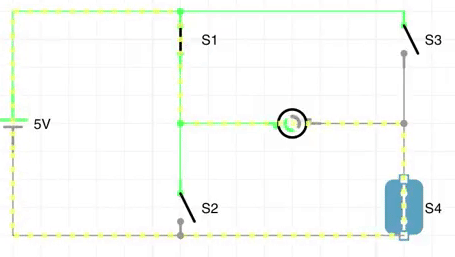
\includegraphics[scale=0.75]{Pictures/Puente_H.PNG}
\caption{Circuito Puente H}
\end{figure}\\

La forma más común de hacer un puente H es usando interruptores de estado sólido ( son llamados transistores ), puesto que sus tiempos de vida y frecuencias de conmutación son mucho más altas. En convertidores de potencia es impensable usar interruptores mecánicos, dado sus especificaciones tan embonables a los requerimientos. Además los interruptores se acompañan de diodos que permitan a las corrientes circular en sentido inverso al previsto cada vez que se conmute la tensión puesto que el motor está compuesto por bobinados que durante varios períodos de tiempo se opondrán a que la corriente varié.

\newpage
\section{Materiales y equipo}
Teniendo en cuenta que utilizaremos el circuito anteriormente visto en la practica pasada, los materiales que faltan serian:\\
* Computadora\\
* Software para simular el circuito\\
* Protoboard \\
* Circuito anterior\\
* Fuente de voltaje\\
* MOSFET's IF540/IF640/IF840\\
* Motor CD\\
* Multímetro\\ 
* Cable para protoboard\\
* Caimanes \\

\newpage
\section{Desarrollo}
\subsection{Realizamos primero la simulación en el software que decidiste utilizar en nuestro caso Proteus, para ver como es su funcionalidad y conexión del puente H, quedando:}
\begin{figure}[hbtp]
\centering
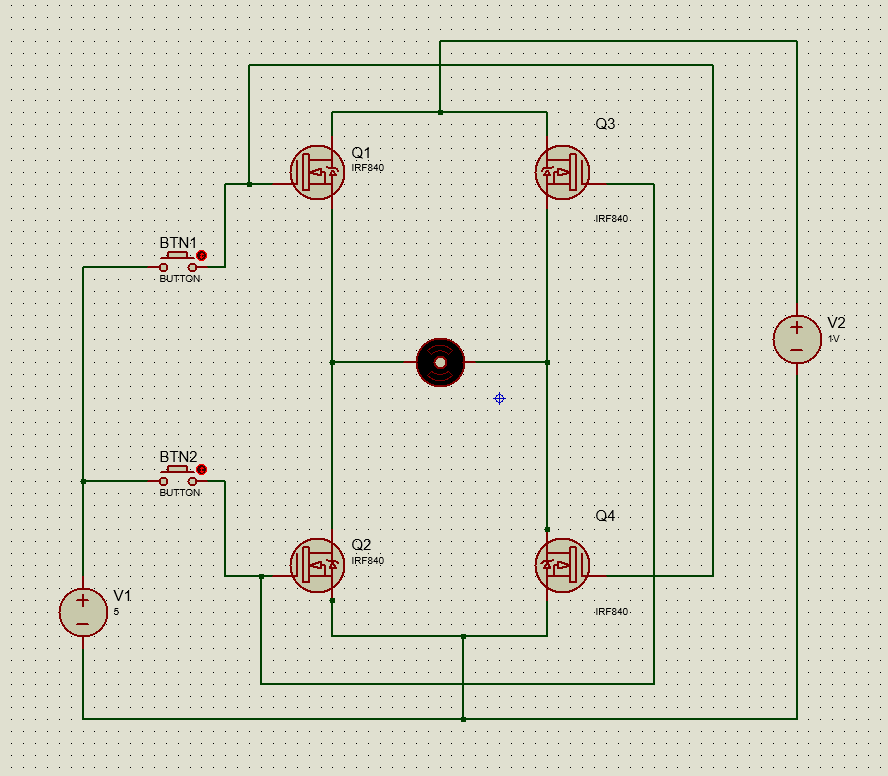
\includegraphics[scale=0.5]{Pictures/Puente.png}
\caption{Simulación Puente H en Proteus}
\end{figure}
En esta simulación observamos que si presionamos un push button el motor empezará a girar para un sentido, si dejamos de presionarlo el motor se detiene; y al presionar el segundo push button el motor gira inversamente al primer movimiento, esto gracias al Puente H con los transistores.

\subsection{El siguiente paso será armar el circuito en el protoboard justo como lo indica la simulación para no cometer errores:}


\subsection{Una vez hecho el circuito del puente vamos a conectarlo a nuestro circuito de la practica pasada:}


\subsection{Metemos el voltaje correspondiente y verificamos que funcione correctamente y que haga bien sus funciones:}

\newpage
\section{Conclusiones}
Cervantez Martinez Luis Osvaldo\\
Bueno para esta practica fue un poco complicada en un inicio por la falta de materiales como lo fue en nuestro caso, ya que no contábamos con resistencias con el valor adecuado para el circuito.\\
Por otra parte, también nos encontramos con varios tropiezos, como fallas y solo nos atoraban más. Lastimosamente por pequeños detalles no pudimos concluir con un circuito muy simple. Ya que el puente h, lo que lo vuelve un poco mas complejo de hacerlo es la obtención de valores de las resistencias a utilizar, las cuales se tienen que conectar en serie con la lampara, esto para facilitar su encendido.\\


Reyes Alvarez Ulises Isaac\\
El Puente H mas que nada nos sirve para controlar un motor, hacerlo girar para el lado que nosotros queremos. Controlado únicamente con dos botones, bueno en nuestro caso utilizando un PLC básico, podemos invertir el giro del motor, hacer que se detenga pero se detendrá bruscamente, algo que esta mal para el motor porque se forza.\\
Con está practica me di una idea bastante genial e interesante que podemos implementarlo en nuestro proyecto o prototipo, para controlar los motores que hacen caminar nuestro prototipo.\\
Su funcionamiento del puente h se debe a los 4 interruptores, mediante 4 transistores que nos ayudan a darle sentido al motor; cuando dos interruptores están cerrados se aplica una tensión haciendo girar el motor en un sentido, al igual al cerrar los otros dos interruptores el voltaje se invierte permitiendo el giro en sentido inverso al motor. 

\newpage
\section{Referencias Bibliográficas}
\url{https://www.ingmecafenix.com/electronica/puente-h-control-motores/}


\end{document}